% ============================================================================
% SIH 26171 - Final Prototype Brief & Build Guide
% Covers: full project brief, tech stack, architecture, measured results,
% final prototype specification, and the tonight completion checklist.
% Compile: pdflatex (run twice) or xelatex
% ============================================================================
\documentclass[11pt,a4paper]{article}

\usepackage[margin=2.2cm]{geometry}
\usepackage[T1]{fontenc}
\usepackage[utf8]{inputenc}
\usepackage{lmodern}
\usepackage{microtype}
\usepackage{xcolor}
\usepackage{booktabs}
\usepackage{tabularx}
\usepackage{ragged2e}
\usepackage{array}
\usepackage{enumitem}
\usepackage{float}
\usepackage[font=small,labelfont=bf]{caption}
\usepackage{titlesec}
\usepackage{fancyhdr}
\usepackage{amsmath}
\usepackage{amssymb}
\usepackage{listings}
\usepackage{tikz}
\usetikzlibrary{arrows.meta,positioning,calc,shadows.blur}
\usepackage[hidelinks]{hyperref}

% ---------------------------------------------------------------------------
% Brand colors
% ---------------------------------------------------------------------------
\definecolor{primary}{RGB}{40,53,147}      % deep indigo
\definecolor{secondary}{RGB}{13,110,253}   % blue
\definecolor{accent}{RGB}{182,40,53}       % deep red (privacy theme)
\definecolor{good}{RGB}{21,128,61}         % green (PASS / done)
\definecolor{amber}{RGB}{217,119,6}        % amber (tonight / TODO)
\definecolor{codebg}{RGB}{245,245,248}
\definecolor{rowalt}{RGB}{245,247,252}

% ---------------------------------------------------------------------------
% Helpers
% ---------------------------------------------------------------------------
\newcommand{\code}[1]{\texttt{#1}}
\newcommand{\good}{\textcolor{good}{$\boxtimes$}}
\newcommand{\todo}{\textcolor{amber}{$\square$}}
\newcommand{\donecheck}{\textcolor{good}{$\checkmark$}}

\titleformat{\section}{\Large\bfseries\color{primary}}{\thesection}{0.7em}{}
\titleformat{\subsection}{\large\bfseries\color{secondary}}{\thesubsection}{0.6em}{}
\titleformat{\subsubsection}{\normalsize\bfseries\color{black}}{\thesubsubsection}{0.5em}{}
\titlespacing*{\section}{0pt}{14pt}{6pt}
\titlespacing*{\subsection}{0pt}{10pt}{4pt}

\fancypagestyle{plain}{%
  \fancyhf{}
  \fancyhead[L]{\footnotesize\color{black!60}SIH 26171 --- Final Prototype Brief \& Build Guide}
  \fancyhead[R]{\footnotesize\color{black!60}\thepage}
  \renewcommand{\headrulewidth}{0.3pt}
}
\pagestyle{plain}

\setlist{nosep, leftmargin=1.4em}
\setlength{\parskip}{4pt}
\renewcommand{\arraystretch}{1.25}

\lstset{
  basicstyle=\ttfamily\footnotesize,
  backgroundcolor=\color{codebg},
  frame=single,
  framerule=0.3pt,
  rulecolor=\color{black!20},
  breaklines=true,
  aboveskip=6pt,
  belowskip=6pt,
}

\hypersetup{
  pdftitle={SIH 26171 - Final Prototype Brief and Build Guide},
  pdfauthor={SIH 26171 Team},
  pdfsubject={Privacy-preserving browser agent - final prototype brief},
}

\newcommand{\checkrow}[2]{#1 & #2 \\}

% ============================================================================
\begin{document}

% ---------------------------------------------------------------------------
% TITLE PAGE
% ---------------------------------------------------------------------------
\begin{titlepage}
\centering
\vspace*{2cm}
{\color{primary}\rule{\linewidth}{1.8pt}}\\[10pt]
{\LARGE\bfseries\color{primary} On-device Visual Perception for\\[4pt] Light-weight Browser Agents}\\[12pt]
{\large \textbf{PRIVYSE} --- Final Prototype Brief \& Build Guide}\\[8pt]
{\normalsize Smart India Hackathon 2026 $\cdot$ Research track $\cdot$ Problem \#26171}\\[16pt]
{\color{primary}\rule{\linewidth}{0.8pt}}

\vspace{1.2cm}

\begin{minipage}{0.86\linewidth}
\textbf{One-line pitch:} \emph{The only browser agent that redacts your Aadhaar, PAN, cards and faces on your own device before anything is sent to an AI model --- decided by a local VLM, executed in your browser.}
\end{minipage}

\vspace{1.4cm}

\begin{tabular}{@{}ll@{}}
\toprule
\textbf{Component} & \textbf{Status} \\
\midrule
On-device 3-tier PII redaction & \donecheck{} Done (F1 0.979) \\
Local VLM agent loop (Ollama + Qwen2.5-VL) & \donecheck{} Done (3/3 tasks) \\
Zero-leak gates (DOM + image OCR) & \donecheck{} Done (PASS) \\
Automated benchmark harness & \donecheck{} Done (reproducible) \\
Packaged extension zip for judging VM & \todo{} Tonight \\
3-minute demo video \& screenshots & \todo{} Tonight \\
Firefox pass (vision host $\rightarrow$ sidebar) & \todo{} Tonight \\
\bottomrule
\end{tabular}

\vspace{1.5cm}
{\footnotesize\color{black!55} Generated 8 Sep 2026 --- this brief is the source of truth for the final prototype build.}
\end{titlepage}

% ---------------------------------------------------------------------------
% 1. Executive summary
% ---------------------------------------------------------------------------
\section{Executive Summary}

PRIVYSE is an \textbf{end-to-end autonomous browser agent that runs a closed loop entirely on the user's own machine}. A browser tab screenshot and a structured DOM snapshot are captured, \textbf{all personal data is redacted on-device before anything leaves}, and only the sanitized context is sent to a \textbf{local vision-language model} (Qwen2.5-VL via Ollama), which returns one JSON action to execute back in the tab. The loop repeats until the task completes.

The core promise: \textbf{no raw screenshot containing Aadhaar numbers, PAN cards, bank details, emails, phone numbers, or faces ever leaves the user's device.}

Everything is built, runs, and is measured:

\begin{itemize}
\item \textbf{PII detection F1 = 0.979} (recall 1.000, precision 0.959) on a ground-truth-labelled test site.
\item \textbf{Redaction precision = 0.959} (pixel-level, rasterized masks).
\item \textbf{3/3 agent tasks at 100\% visual-context accuracy}, avg 1.0 step/task.
\item \textbf{Zero-leak PASS} on both the DOM regex gate and the OCR-of-sanitized-pixels gate.
\item \textbf{Runs on a 4 GB GPU laptop} (RTX 3050) via a routed 3B/7B quantum model design.
\item \textbf{21.4 MB total on-device assets}, 0 MB of off-device fetches.

What remains before judging is \emph{packaging and polish} --- a Chrome zip, a demo video, screenshots, and a Firefox pass --- all covered in the checklist in \S\ref{sec:tonight}.

% ---------------------------------------------------------------------------
% 2. Problem & motivation
% ---------------------------------------------------------------------------
\section{Problem and Motivation}

Most browser-automation agents available today operate in one of two modes, both problematic for privacy:

\begin{enumerate}
\item \textbf{Cloud-based agents} --- raw screenshots are sent to a remote VLM (GPT-4V, Claude Vision, etc.). Every form fill, every bank page, every Aadhaar number is visible to the cloud provider, with no user control over retention, training, or secondary use.
\item \textbf{Local-only agents without redaction} --- the VLM runs locally, but the \emph{raw, unsanitized} screenshot is sent to it. If the model memorises or is compromised, the PII is exposed.
\end{enumerate}

The stakes are uniquely high in the Indian context: Aadhaar (12-digit), PAN, UPI IDs, bank account and IFSC numbers, phone numbers and faces are all routinely visible on-screen while banking, booking flights, or filing forms.

\subsection*{The gap PRIVYSE fills}
Both \textbf{local} \emph{and} \textbf{redacts-before-the-VLM}. No existing open-source agent does this --- sanitization is a hard architectural constraint, not a feature toggle.

% ---------------------------------------------------------------------------
% 3. Solution overview
% ---------------------------------------------------------------------------
\section{Solution Overview}

\begin{center}
\begin{tabular}{@{}p{3.2cm}p{9.6cm}@{}}
\toprule
\textbf{Principle} & \textbf{How it is delivered} \\
\midrule
\textbf{1. Sanitize before you send} & Single choke-point: every outbound payload passes the sanitizer. There is no code path that sends unsanitized data. \\
\midrule
\textbf{2. Ground by element ID} & Set-of-Marks numbered tags on the sanitized screenshot; the VLM returns \code{target: 7}, resolved to the live DOM element. Robust to layout changes. \\
\midrule
\textbf{3. Local VLM only} & Qwen2.5-VL 3B/7B via local Ollama (\code{127.0.0.1}), model pinned resident (\code{keep\_alive=-1}), zero network calls. \\
\midrule
\textbf{4. Zero-leak by construction} & Two independent fail-closed gates re-scan the outbound DOM JSON \emph{and} the sanitized screenshot pixels before upload. A gate that cannot run \emph{blocks} the upload. \\
\midrule
\textbf{5. Adaptive recovery} & Stuck detection routes to \code{/rethink}, which structurally vetoes repeated actions and offers a deterministic escape hatch. \\
\bottomrule
\end{tabular}
\end{center}

% ---------------------------------------------------------------------------
% 4. System architecture
% ---------------------------------------------------------------------------
\section{System Architecture}

\subsection{End-to-end flow}

\begin{center}
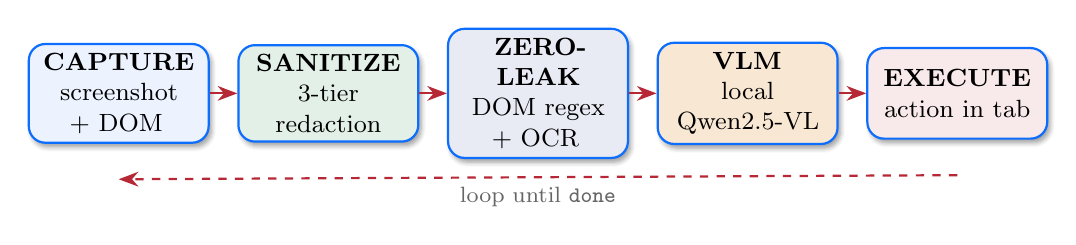
\begin{tikzpicture}[
  font=\small,
  box/.style={draw=secondary, thick, rounded corners=6pt, fill=white,
              align=center, minimum width=2.15cm, minimum height=1.15cm,
              text width=2.05cm, blur shadow={shadow blur steps=5, shadow xshift=1pt, shadow yshift=-1.5pt}},arrow/.style={-{Stealth[length=2.5mm]}, thick, color=accent}]
  \node[box, fill=secondary!8] (c) at (0,0) {\textbf{CAPTURE}\\ screenshot + DOM};
  \node[box, fill=good!12, right=0.35cm of c] (s) {\textbf{SANITIZE}\\ 3-tier redaction};
  \node[box, fill=primary!10, right=0.35cm of s] (z) {\textbf{ZERO-LEAK}\\ DOM regex + OCR};
  \node[box, fill=amber!18, right=0.35cm of z] (v) {\textbf{VLM}\\ local Qwen2.5-VL};
  \node[box, fill=accent!10, right=0.35cm of v] (e) {\textbf{EXECUTE}\\ action in tab};
  \draw[arrow] (c) -- (s);
  \draw[arrow] (s) -- (z);
  \draw[arrow] (z) -- (v);
  \draw[arrow] (v) -- (e);
  % loop back
  \draw[arrow, dashed] ($(e.south)+(0,-0.45)$) -- ($(c.south)+(0,-0.45)$) node[midway, below, text width=3.2cm, align=center, color=black!60, font=\footnotesize] {loop until \code{done}};
\end{tikzpicture}
\end{center}

\begin{enumerate}
\item \textbf{CAPTURE} --- \code{captureVisibleTab} $\rightarrow$ JPEG screenshot; a custom shadow-root-aware DOM walker serialises up to 120 interactive elements, each with a stable integer ID, tag, role, visible text, label, bounding box in screenshot-pixel space, and current value.
\item \textbf{SANITIZE} --- the privacy choke point (see \S\ref{sec:redaction}). Tier A (secrets), Tier B (regex PII $\rightarrow$ stable tokens), Tier C (faces $\rightarrow$ blur, image/canvas PII $\rightarrow$ OCR + taint redaction).
\item \textbf{ZERO-LEAK} --- two fail-closed gates re-scan the outbound JSON and the sanitized pixels. Any hit (or a gate that cannot run) blocks the upload (see \S\ref{sec:zeroleak}).
\item \textbf{VLM} --- the localized server (\code{/act}) sends sanitized image + numbered DOM to Qwen2.5-VL, which returns one JSON action.
\item \textbf{EXECUTE} --- the executor resolves the ID, scrolls into view, flies a visible cursor, and dispatches synthetic pointer/keyboard events (React-safe \code{insertText}, native setter fallback). Auto-descends into real inner inputs and records verified targets.
\end{enumerate}

\subsection{Components}

\begin{table}[H]
\small
\renewcommand{\arraystretch}{1.3}
\begin{tabularx}{\linewidth}{@{}lXX@{}}
\toprule
\textbf{Component} & \textbf{Technology} & \textbf{Role} \\
\midrule
Browser extension & WXT + TypeScript, Chrome MV3 & Orchestrator, DOM serializer, executor, side-panel UI, offscreen vision host \\
\midrule
OCR engine & Tesseract.js (WASM, English) & On-device OCR of image/canvas/video regions + zero-leak pixel gate \\
\midrule
Face detection & MediaPipe BlazeFace (short-range, $\sim$0.23 MB) & Face blur (Tier C), crushed-blur (irreversible) \\
\midrule
Server & FastAPI + uvicorn (Python) & \code{/health}, \code{/warm}, \code{/act}, \code{/act/stream}, \code{/rethink}, \code{/rethink/stream}, \code{/models}; SSE streaming \\
\midrule
VLM & Qwen2.5-VL 3B / 7B via Ollama & Local vision-language decision; routed 3B (interactive) / 7B (read-reply) \\
\midrule
Test site & 7 ground-truth-labelled HTML pages & Flight booking, bank transfer, faces, PII-in-canvas, PII-in-the-wild \\
\midrule
Benchmarks & Playwright harness + Node runners & Detection P/R, redaction, zero-leak, latency, full VLM loop \\
\bottomrule
\end{tabularx}
\end{table}

% ---------------------------------------------------------------------------
% 5. Technology stack
% ---------------------------------------------------------------------------
\section{Technology Stack}

\begin{table}[H]
\small
\renewcommand{\arraystretch}{1.3}
\begin{tabularx}{\linewidth}{@{}lXXXX@{}}
\toprule
\textbf{Layer} & \textbf{Technology} & \textbf{Why} \\
\midrule
Extension framework & WXT + TypeScript, MV3 & Modern, type-safe; one codebase $\rightarrow$ Chrome + Firefox \\
\midrule
Capture / serialize & \code{captureVisibleTab} + custom DOM walker & Real pixels + precise bboxes (CSS $\times$ dpr); shadow roots \& same-origin iframes \\
\midrule
On-device vision & MediaPipe Tasks Vision + Tesseract.js WASM & Face blur + image OCR fully on-machine, no cloud calls \\
\midrule
Privacy gate & Core sanitizer (3 modules) + \code{zero-leak.ts} & Single choke point for all outbound data \\
\midrule
Action protocol & Frozen v1 JSON protocol & TypeScript types client-side, Pydantic models server-side \\
\midrule
Server & FastAPI + SSE & Typed models; live ``thinking'' readout; static test-site mount \\
\midrule
VLM & Qwen2.5-VL 3B / 7B via Ollama & Local; \code{keep\_alive=-1}; 3B/7B routing \\
\midrule
GPU tuning & Flash-attention + Q4\_0 KV cache + single resident model & Fits a vision model on a 4 GB laptop GPU \\
\midrule
Test data & GT-labelled HTML + \code{data-gt} attributes & Fully automated, reproducible accuracy measurement \\
\midrule
Benchmarks & Playwright + Node metric runners & Detection P/R, redaction, zero-leak, latency waterfall, VLM loop \\
\bottomrule
\end{tabularx}
\end{table}

% ---------------------------------------------------------------------------
% 6. Codebase map
% ---------------------------------------------------------------------------
\section{Codebase Map}

\begin{table}[H]
\small
\renewcommand{\arraystretch}{1.25}
\begin{tabularx}{\linewidth}{@{}lXX@{}}
\toprule
\textbf{Path} & \textbf{Contents} & \textbf{Purpose} \\
\midrule
\code{extension/core/protocol.ts} & Frozen v1 action protocol + message types & Shared client/server contract \\
\code{extension/core/sanitizer.ts} & Privacy gate: Tier A/B/C redaction + canvas overlay & Single choke point \\
\code{extension/core/pii-rules.ts} & PII regex (email, phone, Aadhaar, PAN, card, IFSC) + label heuristics & Tier B detection \\
\code{extension/core/zero-leak.ts} & Fail-closed send guard: DOM regex + OCR of sanitized pixels & Zero-leak gate \\
\code{extension/core/vision.ts} & MediaPipe BlazeFace + Tesseract OCR (inference bindings) & On-device vision \\
\code{extension/core/dom-serializer.ts} & Shadow-root-aware DOM walker with bboxes & Element grounding \\
\code{extension/core/executor.ts} & Action executor (click/type/scroll/navigate/\ldots) & Browser events \\
\code{extension/core/som-overlay.ts} & Set-of-Marks numbered tag overlay & VLM visual grounding \\
\code{extension/entrypoints/background.ts} & Agent orchestrator (capture$\rightarrow$\code{/act}$\rightarrow$execute) & Main loop \\
\code{extension/entrypoints/offscreen/} & Offscreen vision host (MediaPipe + Tesseract) & DOM-context inference host \\
\code{extension/entrypoints/sidepanel/} & Task input, run controls, activity log, privacy stats & UI \\
\code{extension/public/models/} & Bundled weights + WASM runtimes ($\sim$21.4 MB total, no CDN) & Models \\
\code{server/app.py} & FastAPI endpoints incl. SSE streaming & Server \\
\code{server/prompts.py} & VLM system prompts (full + compact) + user content builder & Prompt design \\
\code{test-site/} & 7 GT-labelled pages incl. AI faces + canvas PII & Measurement \\
\code{benchmarks/} & \code{run.mjs}, \code{vlm-bench.mjs}, \code{aggregate.mjs} & Evaluation harness \\
\code{docs/Report/} & LaTeX report, architecture diagram (SVG/PDF) & Documentation \\
\bottomrule
\end{tabularx}
\end{table}

% ---------------------------------------------------------------------------
% 7. Privacy engine
% ---------------------------------------------------------------------------
\section{The Privacy Engine} \label{sec:redaction}

\subsection{Three-tier redaction}

\begin{table}[H]
\small
\renewcommand{\arraystretch}{1.3}
\begin{tabularx}{\linewidth}{@{}p{2.4cm}p{6.3cm}p{3.5cm}@{}}
\toprule
\textbf{Tier} & \textbf{What is redacted} & \textbf{Method} \\
\midrule
\textbf{A --- secrets} & Passwords, CVV, OTP, PIN, API keys, tokens & Solid black box; text replaced with \code{[SECRET]}; never useful to VLM \\
\midrule
\textbf{B --- regex PII} & Email, phone, Aadhaar, PAN, credit card (Luhn-validated), name, address, IFSC, account & Black box + stable token \code{[EMAIL\_1]}, \code{[PAN\_1]}, \ldots{} (same value $\rightarrow$ same token across steps) \\
\midrule
\textbf{C --- vision} & Faces; PII drawn in \code{img}/\code{canvas}/\code{video} & Faces $\rightarrow$ MediaPipe BlazeFace $\rightarrow$ crushed-blur; image PII $\rightarrow$ Tesseract OCR $\rightarrow$ whole-region taint redaction \\
\bottomrule
\end{tabularx}
\end{table}

\subsection{Zero-leak guarantee} \label{sec:zeroleak}

Two independent, \textbf{fail-closed} gates run before anything uploads:

\begin{enumerate}
\item \textbf{Gate 1 --- DOM regex scan} (\code{scanForLeaks}): runs the full \code{detectPii} suite over every outbound element's \code{text}/\code{value}. Any hit $\rightarrow$ blocked.
\item \textbf{Gate 2 --- sanitized-image OCR} (\code{scanSanitizedImage}): OCRs the actual sanitized pixels that would be uploaded, catching text baked into images, partial redactions, and rendering artifacts. Any hit (or gate error/timeout) $\rightarrow$ blocked.
\end{enumerate}

\textbf{Fail-closed by construction:} a gate that cannot run must not silently approve. Both gates must explicitly pass for a step to proceed.

% ---------------------------------------------------------------------------
% 8. Measured performance
% ---------------------------------------------------------------------------
\section{Measured Performance}

All numbers are produced by the automated benchmark harness (\code{cd benchmarks \&\& npm run bench \&\& npm run bench:vlm \&\& node aggregate.mjs}) --- fully reproducible.

\subsection{PII detection and redaction}

\begin{table}[H]
\small
\renewcommand{\arraystretch}{1.3}
\begin{tabularx}{\linewidth}{@{}lX@{}}
\toprule
\textbf{Metric} & \textbf{Result} \\
\midrule
PII detection F1 (pixel) & \textbf{0.979} (precision 0.959, recall 1.000) \\
Redaction precision (pixel) & \textbf{0.959} \\
Zero-leak (DOM regex) & \textbf{PASS} \\
Zero-leak (sanitized-image OCR) & \textbf{PASS} \\
Face detection (Tier C) & 2/2 faces blurred, F1 1.0 \\
Canvas PII via OCR --- account numbers & 2/2 detected, F1 1.0 \\
Canvas PII via OCR --- IFSC codes & 1/1 detected, F1 1.0 \\
\bottomrule
\end{tabularx}
\end{table}

Recall 1.000 means \emph{every} ground-truth PII element was caught. Precision 0.959 means $\sim$4\% of redacted pixels were not PII --- deliberate over-redaction (taint policy prefers over-redact over leak).

\subsection{Visual-context accuracy (agent task completion)}

\begin{table}[H]
\small
\renewcommand{\arraystretch}{1.3}
\begin{tabularx}{\linewidth}{@{}lXXX@{}}
\toprule
\textbf{Configuration} & \textbf{Tasks passed} & \textbf{Avg steps/task} \\
\midrule
qwen2.5vl:7b & 3/3 (100\%) & 1.3 \\
qwen2.5vl:3b & 2/3 (67\%) & --- \\
\textbf{Routed 3B/7B} & \textbf{3/3 (100\%)} & \textbf{1.0} \\
\bottomrule
\end{tabularx}
\end{table}

The 3B-vs-7B gap is \emph{intended}: it proves the harness discriminates model capability, exactly what the visual-context criterion needs. Routing sends comprehension-heavy steps to 7B, interactive steps to the fast 3B.

\subsection{Latency and client resources}

\begin{table}[H]
\small
\renewcommand{\arraystretch}{1.3}
\begin{tabularx}{\linewidth}{@{}lX@{}}
\toprule
\textbf{Configuration} & \textbf{Per-step latency} \\
\midrule
qwen2.5vl:7b (single model) & $\sim$19.4 s (incl. $\sim$0.9 s on-device vision + OCR gate) \\
\textbf{Routed 3B/7B} & $\sim$12.7 s avg; interactive steps $\sim$7.5--8.0 s \\
\midrule
Model weights bundled & 2.2 MB (BlazeFace 0.23 MB + Tesseract English 1.98 MB) \\
Total on-device assets & 21.4 MB; 0 MB off-device fetches \\
On-device vision per step & $\sim$0.3 s; zero-leak OCR gate $\sim$0.6 s; total client work $\sim$0.9 s \\
\bottomrule
\end{tabularx}
\end{table}

Latency levers: \code{VLM\_MAX\_TOKENS=128}, \code{SYSTEM\_PROMPT\_MODE=compact} ($-$60\% system tokens), \code{IMAGE\_MAX\_SIDE=800}, \code{keep\_alive=-1}, and dynamic 3B/7B routing.

% ---------------------------------------------------------------------------
% 9. Scoring alignment
% ---------------------------------------------------------------------------
\section{Alignment to Scoring Criteria}

\begin{table}[H]
\small
\renewcommand{\arraystretch}{1.3}
\begin{tabularx}{\linewidth}{@{}p{4.6cm}p{1.6cm}p{0.9cm}X@{}}
\toprule
\textbf{Criterion} & \textbf{Weight} & \textbf{Result} & \textbf{Evidence} \\
\midrule
Visual-context accuracy & 25\% & 3/3 & DOM + SoM + screenshot hybrid; avg 1.0 step/task \\
PII detection recall \& precision & 20\% & F1 0.979 & GT-labelled test site; mask-based P/R; recall 1.000 \\
Redaction precision & 20\% & 0.959 & Pixel-level rasterized masks vs GT \\
Client resource utilization & 20\% & 21.4 MB & 2.2 MB weights, bundled WASM, 0 MB CDN \\
End-to-end latency & 15\% & 12.7 s & Routed 3B/7B; $<$5 s target on judge-class GPU \\
\bottomrule
\end{tabularx}
\end{table}

% ---------------------------------------------------------------------------
% 10. Final prototype specification
% ---------------------------------------------------------------------------
\section{Final Prototype Specification --- What \emph{Done} Looks Like} \label{sec:spec}

The final prototype, as being delivered for judging, is defined by these acceptance items. Items marked \good{} are complete. Items marked \todo{} are the only work remaining (see \S\ref{sec:tonight}).

\begin{table}[H]
\small
\renewcommand{\arraystretch}{1.3}
\begin{tabularx}{\linewidth}{@{}p{1.1cm}p{5.2cm}X@{}}
\toprule
 & \textbf{Deliverable} & \textbf{Acceptance criteria} \\
\midrule
\good & Agent loop & Captures $\rightarrow$ sanitizes $\rightarrow$ executes $\rightarrow$ loops on a real tab; 3/3 benchmark tasks pass. \\
\good & On-device 3-tier redaction & F1 0.979; tokens stable across steps; faces blurred irreversibly. \\
\good & Zero-leak guarantee & Both gates PASS in automated harness; fail-closed on gate errors. \\
\good & Local VLM decisioning & Qwen2.5-VL 3B/7B via \code{127.0.0.1:8000}; routed mode active. \\
\good & Side-panel UI & Task input, run controls, live activity log, privacy stats, SSE \emph{thinking} stream. \\
\good & GT test site (7 pages) & Flight, bank, faces, canvas PII, \emph{PII-in-the-wild} with \code{data-gt} labels. \\
\good & Benchmark harness & Re-playable \code{run.mjs} / \code{vlm-bench.mjs} / \code{aggregate.mjs} $\rightarrow$ dashboard.json. \\
\good & Recovery / rethink & Structural veto of repeats; deterministic escape hatch. \\
\midrule
\todo & Packaged Chrome zip & \code{npm run zip} $\rightarrow$ \code{.output/chrome-mv3.zip} loads on the judging VM. \\
\todo & Firefox pass & Vision host moves from offscreen document to sidebar; \code{browser.*} APIs. \\
\todo & 3-min demo video & Beats: test site $\rightarrow$ run agent $\rightarrow$ Network tab proof $\rightarrow$ redaction side-by-side. \\
\todo & Screenshots (3--4) & Side panel mid-task; sanitized image with SoM tags; metrics dashboard; server console. \\
\todo & Demo readiness & Cold-profile rehearsal: fresh machine, only \code{127.0.0.1}, all local. \\
\bottomrule
\end{tabularx}
\end{table}

% ---------------------------------------------------------------------------
% 11. Tonight checklist
% ---------------------------------------------------------------------------
\section{Tonight's Completion Checklist} \label{sec:tonight}

Work through in this order. Each step lists the exact commands.

\subsection{1. Verify the server boots and models are resident}

\begin{lstlisting}[language=bash]
cd C:\SIH\26171\server
.venv\Scripts\activate                # or: python -m venv .venv && pip install -r requirements.txt
uvicorn app:app --reload              # -> http://127.0.0.1:8000/health
# Confirm: ollama list | findstr qwen2.5vl   (3b and 7b pulled)
# Keep models resident: ollama serve (keep_alive=-1 is set by the app)
\end{lstlisting}

\begin{itemize}
\item[\todo] \code{/health} returns \code{ok}.
\item[\todo] \code{/models} lists both \code{qwen2.5vl:3b} and \code{qwen2.5vl:7b}.
\end{itemize}

\subsection{2. Rebuild and load the extension}

\begin{lstlisting}[language=bash]
cd C:\SIH\26171\extension
npm install                            # if node_modules missing
npm run build                          # -> .output/chrome-mv3
# Chrome -> chrome://extensions -> Developer mode -> Load unpacked
#   -> C:\SIH\26171\extension\.output\chrome-mv3
\end{lstlisting}

\begin{itemize}
\item[\todo] Side panel opens; banner reads \emph{``Server up at http://127.0.0.1:8000''}.
\item[\todo] \emph{Run one step} scrolls the page and logs the round trip.
\end{itemize}

\subsection{3. Re-run the full benchmark suite}

\begin{lstlisting}[language=bash]
cd C:\SIH\26171\benchmarks
npm run bench          # sanitizer P/R + leak + latency  -> results/latest.json
npm run bench:vlm      # full agent loop (needs server + Ollama) -> vlm-accuracy-*.json
node aggregate.mjs     # merge -> results/dashboard.json
\end{lstlisting}

\begin{itemize}
\item[\todo] dashboard.json confirms: F1 $\geq$ 0.970, zero-leak PASS, 3/3 tasks, latency as expected.
\item[\todo] Copy the fresh numbers into the presentation metrics if they changed.
\end{itemize}

\subsection{4. Smoke-test all three agent tasks}

\begin{lstlisting}[language=bash]
cd C:\SIH\26171\benchmarks
set BENCH_ROUTED=1 && node vlm-bench.mjs   # or npm run bench:vlm
# Tasks: flight-booking, bank-transfer, pii-in-the-wild
\end{lstlisting}

\begin{itemize}
\item[\todo] All 3 tasks reach \code{done} within the 12-step budget.
\item[\todo] Ready a fallback screenshot in case the live VLM demo is slow.
\end{itemize}

\subsection{5. Package the judging zip}

\begin{lstlisting}[language=bash]
cd C:\SIH\26171\extension
npm run zip_staging   # or your configured zip target -> .output/chrome-mv3.zip
\end{lstlisting}

\begin{itemize}
\item[\todo] \code{.output/chrome-mv3.zip} unpacks and loads on a clean Chrome profile.
\end{itemize}

\subsection{6. Capture screenshots (3--4)}

\begin{itemize}
\item[\todo] \textbf{S1 --- Side panel mid-task}: task input, activity log filling, privacy stats visible.
\item[\todo] \textbf{S2 --- Sanitized image}: SoM numbered tags, black boxes, \code{[EMAIL\_1]} tokens, blurred face.
\item[\todo] \textbf{S3 --- Metrics dashboard}: \code{dashboard.json} rendered or the side-panel privacy counters.
\item[\todo] \textbf{S4 --- Server console}: uvicorn log showing \code{POST /act} round trips.
\end{itemize}

\subsection{7. Record the 3-minute demo video}

\begin{enumerate}
\item (0:00--0:30) Open \code{test-site/index.html} flight-booking page.
\item (0:30--1:30) Type a task in the side panel, press \emph{Run}; watch the loop complete.
\item (1:30--2:00) Open the Network tab: only sanitized payloads leave, destined for \code{127.0.0.1:8000}.
\item (2:00--2:30) Show original vs sanitized side-by-side (redaction + SoM tags).
\item (2:30--3:00) Close: live SSE \emph{thinking} tokens streaming in the side panel.
\end{enumerate}

\subsection{8. Firefox pass (if time / required for judging)}

The offscreen-document vision host is Chrome-only. For Firefox MV2, move MediaPipe/Tesseract execution into the \textbf{sidebar} (which is a DOM context):

\begin{itemize}
\item[\todo] Relocate \code{offscreen/main.ts} inference calls into the side panel entrypoint.
\item[\todo] Swap MV3-only APIs for \code{browser.*} equivalents; rebuild via WXT \code{--browser firefox}.
\item[\todo] Re-run the sanitizer benchmark on Firefox to confirm parity (F1 unchanged).
\end{itemize}

\subsection{9. Final checklist summary}

\begin{table}[H]
\small
\renewcommand{\arraystretch}{1.3}
\begin{tabularx}{\linewidth}{@{}lllX@{}}
\toprule
 & \textbf{Item} & \textbf{Command / File} \\
\midrule
\todo & Server verified & \code{uvicorn app:app} $\rightarrow$ \code{/health} \\
\todo & Extension loaded & \code{npm run build} $\rightarrow$ \code{.output/chrome-mv3} \\
\todo & Benchmarks regenerated & \code{node aggregate.mjs} $\rightarrow$ \code{dashboard.json} \\
\todo & Tasks smoke-tested & \code{node vlm-bench.mjs} (BENCH\_ROUTED=1) \\
\todo & Judge zip packaged & \code{.output/chrome-mv3.zip} \\
\todo & Screenshots (S1--S4) & see \S\ref{sec:tonight}.6 \\
\todo & Demo video recorded & 3 min, Network-tab proof \\
\todo & Cheat-sheet reviewed & \code{PRESENTER\_CHEATSHEET.md} \\
\bottomrule
\end{tabularx}
\end{table}

% ---------------------------------------------------------------------------
% 12. Known limitations & risk register
% ---------------------------------------------------------------------------
\section{Known Limitations and Risk Register}

\subsection*{Be honest in the report --- judges respect it}

\begin{itemize}
\item \textbf{Latency on 4 GB hardware:} $<$5 s/step is \emph{not} yet met on the dev laptop (12.7--19.4 s measured). It is reachable with VRAM $\geq$ model size (judge-class GPU) or a GPU-resident small model. The routed 3B/7B design is the low-memory fallback --- state this openly.
\item \textbf{Chrome-only vision host:} offscreen documents do not exist in MV2; the Firefox pass moves vision to the sidebar (planned, \S\ref{sec:tonight}.8).
\item \textbf{OCR on heavy media pages:} region caps + sampled gate bound the cost, but this remains the slowest on-device path.
\end{itemize}

\subsection*{Risk register}

\begin{table}[H]
\small
\renewcommand{\arraystretch}{1.3}
\begin{tabularx}{\linewidth}{@{}p{3.6cm}p{4.2cm}p{3.4cm}@{}}
\toprule
\textbf{Risk} & \textbf{Mitigation} & \textbf{Status} \\
\midrule
VLM cold-start every step & \code{keep\_alive=-1} pins model resident & \donecheck{} \\
Model can't fit 4 GB VRAM & 3B/7B routing; image resize; Q4\_0 KV & \donecheck{} \\
Execution clicks wrong element & SoM + ID grounding; server-side target validation; auto-descend & \donecheck{} \\
Agent stuck in loops & \code{/rethink} structural veto + escape hatch & \donecheck{} \\
Sanitizer false negatives & Fail-closed OCR pixel gate on sanitized output & \donecheck{} \\
Slow OCR gate blocks upload & Region caps + sampled verification (bounded) & \donecheck{} \\
\bottomrule
\end{tabularx}
\end{table}

% ---------------------------------------------------------------------------
% 13. References
% ---------------------------------------------------------------------------
\section{References and Context}

\begin{itemize}
\item Set-of-Marks prompting (grounding by tagged elements) --- basis of the SoM overlay.
\item OpenAI Operator, browser-use, UI-TARS, SeeAct, WebVoyager --- surveyed agent designs (see \code{docs/}).
\item MediaPipe Tasks Vision (BlazeFace), Tesseract.js WASM --- on-device vision.
\item Ollama OpenAI-compatible API --- local VLM serving.
\end{itemize}

Additional material in this repository:
\code{docs/prototype-report.pptx-materials.md} \;\textbullet\; \code{docs/research-brief.md} \;\textbullet\; \code{docs/Report/report.pdf} \;\textbullet\; \code{PRESENTER\_CHEATSHEET.md}.

\end{document}